% Objecthood as a composition of differentiae; scaling the world model with the
% network of modulating zones. Build:
%   pdflatex manipulator && bibtex manipulator && pdflatex manipulator && pdflatex manipulator
\documentclass[11pt]{article}

\usepackage[margin=1in]{geometry}
\usepackage{graphicx}
\usepackage{amsmath}
\usepackage{booktabs}
\usepackage{microtype}
\usepackage[numbers,sort&compress]{natbib}
\usepackage[colorlinks=true,allcolors=blue]{hyperref}

\graphicspath{{../figures/}}

\title{\textbf{Objecthood as a composition of differentiae:\\ scaling the world model with a network of modulating zones\\ in an embodied Sensation Modulating Network}}
\author{G.\ Nagarjuna\thanks{IISER Pune, India.} \and Durgaprasad Karnam\thanks{IIT Bombay, India.}}
\date{\today}

\begin{document}
\maketitle

\begin{abstract}
\noindent
An agent's grip on its world is usually derived either by training a world-model
on data or by inverting an internal generative model. We pursue a third route,
from the Sensation Modulating Network (SMN): in a body built as a \emph{network
of opponent, pull-only, dual-interface zones} immersed in a real gravitational
field, the rudiments of objecthood, agency, and directedness are \emph{enacted by
construction}. We make one thesis precise and falsifiable on a physics-engine
bench. A single zone registers a \emph{difference} along its line of modulation
--- a \emph{differentia} --- not yet an object: it reports how a thing answers the
agent's own pull (objecthood-as-resistance), factors \textbf{self / field /
object} through a force-reafference model that predicts its own effort against
gravity, and sustains a halt that is persistent, returnable, and side-specific
(directedness). An \emph{object} is a \emph{composition of differentiae}, and
composition requires a \emph{network} of zones coupled through the modulatory
board. We then show the clinching result: the agent's world-model capacity ---
the objects it can individuate --- scales as $2^{K}$ with the number of zones the
network binds (verified against real multi-zone presses), while zones present but
\emph{unbound} add nothing. The world model is built by the \emph{network}, not by
the sensor count: scaling the modulation is scaling the world, and its onset is a
\emph{percolation-like transition} in the network's coupling density. Everything
is reproducible from an open bench.
\end{abstract}

\section{Introduction}

How does an agent come to have a world of objects it can act on, to tell its own
doings from the world's, and to be \emph{about} something? Two answers dominate.
The machine-learning answer trains a world-model from a corpus
\citep{Chen2018NeuralODE}. The active-inference answer equips the agent with an
internal generative model and minimizes prediction error by inferring hidden
causes \citep{ParrPezzuloFriston2022}. Both place the structuring prior
\emph{inside} the agent.

We pursue a third route, from the SMN architecture \citep{NagarjunaKarnam2026SMN}.
An SMN agent is a network of \emph{opponent, dual-interface zones}: each zone acts
through a pull-only antagonist pair and senses, through the same interface, the
effort and contact that pull meets. The agent is immersed in a real physical
field and reads that field \emph{only through the work it does against it}. On
this view the structuring prior is not in the head but in the world--body
coupling --- gravity is a strong, free prior --- and the agent's grip on its
world is \emph{enacted by construction}, neither learned from data nor inferred
over a model.

Our central claim is a claim about \emph{composition and scale}. A single zone
registers a \emph{difference} along one line of modulation --- a \emph{differentia}
in the classical sense, a ``difference that makes a difference''
\citep{Bateson1972}. A difference is not an object. An \emph{object} is a
\emph{composition} of differentiae (Aristotle's genus-plus-differentiae; a convex
region across several domains \citep{Gardenfors2014}), and to compose differentiae
the body must \emph{couple} its zones --- it must be a network. This dissolves an
obvious objection (``where is the network?''): the body \emph{is} the network, and
the world it can construct grows with it. Four results, none requiring any
training, develop the claim on a contact bench:

\begin{enumerate}
\item \textbf{A single zone is a difference register.} Pressing on a thing, one
  zone reads how it answers the pull --- a force$\to$result mapping that separates
  objects by resistance, the one differentia the zone affords.
\item \textbf{Self, field, and object are factored architecturally}, by a
  force-reafference model that predicts the agent's own effort against the field.
\item \textbf{Haltability generates aboutness}: that single-zone register can hold
  a directed, returnable, side-specific halt --- the body's way of being about a
  thing.
\item \textbf{Objecthood is a composition of differentiae, and it scales with the
  network.} Coupling $K$ zones through the board composes $K$ differentiae into an
  object; the world-model capacity scales as $2^{K}$ with the \emph{bound}
  network, not with the raw sensor count.
\end{enumerate}

\section{Background: differences, forces, and the construction of objects}

That objects are \emph{composed} of differences is an old thought made precise in
several traditions. \citet{Bateson1972} took the elementary unit of mind to be a
``difference that makes a difference''; classically an object is individuated by
its \emph{differentiae}; and \citet{Gardenfors2014} models an object category as a
convex region across \emph{several} quality domains --- a composition of
differences, one per domain. That objects are not \emph{given} but
\emph{constructed} --- wrestled from a flux by an engaged subject through what
\citet{Smith1996} calls \emph{registration}, a deliberate middle course between
realism and constructionism --- is the metaphysical companion of the same thesis.
Our contribution is a minimal, sub-semantic, embodied mechanism for it:
differences are registered by single zones, objects by their composition across a
coupled network.

The single-zone differentia we report is force-based. Following
\citeauthor{Gardenfors2020}'s two-vector model of events
\citep{Gardenfors2020,GardenforsWarglien2012}, an event is an action \emph{force
vector} mapped to a \emph{result vector}; friction and gravity enter as
\emph{counterforces} \citep{Talmy1988,Wolff2007}. Our zone enacts that mapping ---
the antagonist pull is the force, the thing's response is the result, the field is
the counterforce --- by construction rather than by learning. Recurrent dynamical
systems can be \emph{trained} to categorize \citep{Beer2003,Maass2002}; we do not
train. Active inference \citep{ParrPezzuloFriston2022,PezzuloCisek2016} locates the
prior in a represented model; we locate it in the world--body coupling.
\citet{Brooks1991} rejected dataset and representation alike but reached a ceiling
at higher cognition; we keep the no-dataset commitment while adding the modulation
that \emph{binds} differentiae into objects. Morphological computation
\citep{PfeiferBongard2006} and the sensorimotor/ecological tradition
\citep{ORegan2001,Gibson1979} are allies throughout.

\section{The bench: zones, the basal floor, and the board}

The experiments run on \texttt{smn-lab}, an open MuJoCo bench in which the SMN
control architecture drives a physical body \citep{NagarjunaKarnam2026SMN}. The
atom is a \textbf{zone}: a degree of freedom driven by a \emph{pull-only
antagonist pair} --- there are no position (``stepper'') commands; the agent
modulates two opposing pulls, whose co-activation is the atomic equilibrium we
call a \emph{balance}. Each zone's \textbf{dual interface} reads joint state, the
actuator effort (the work the pull performs), and contact. Beneath the zones runs
the \textbf{basal action pattern generator (BAPG)}: not a \emph{central} pattern
generator but the architecture's distributed, evolutionarily ancient innermost
\emph{floor}, an endogenous drive the higher layers gate. The BAPG supplies the
continuous modulation that fills the spaces \emph{between} the discrete
differentiae, which is why the constructed world is not pixelated: it is generated
by coupled dynamical systems, not by linear algebra.

Zones are wired by the \textbf{board} (the ``balance beam''), the coupling network
that lets one zone's reading enter another's --- the substrate of composition. A
\emph{single} zone has a trivial board; objecthood, as a composition of
differentiae, requires a non-trivial one. The body's structure fixes, \emph{a
priori}, a finite \textbf{register lattice} (Contact $\times$ Effort $\times$
Motion per zone) --- the space of distinctions the agent can occupy --- and an
experiment records which subset it occupies. Gravity is on, the floor frictional,
and objects carry mass, fixation, and compliance; the agent reads the field
through effort. A single-joint probe confirmed the read separates free, movable,
compliant, and fixed targets cleanly (not shown).

\section{Results}

\subsection{E1 --- a single zone is a difference register}

A zone presses five things differing only in how they answer the pull: \emph{free},
\emph{movable-light}, \emph{movable-heavy}, \emph{compliant}, \emph{fixed}. Each is
summarized by the contact \emph{impulse} it returns (resistance) and the angle the
limb reaches (yielding). The five fall on a single monotone arc
(Figure~\ref{fig:e1}, Table~\ref{tab:e1}) --- a force$\to$result mapping that
registers one \emph{differentia}, resistance-to-modulation. This is honestly a
\emph{difference register}, not yet objecthood: along one line of modulation the
zone tells things apart, but it composes nothing. Driven instead by a position
(``stepper'') controller commanded to an angle, the body \emph{overpresses what it
cannot reach}: on the fixed thing its contact impulse is $57$\,N\,s versus the SMN
pull's $19$ --- the unbounded failure of commanding an angle rather than modulating
a force.

\begin{table}[t]
  \centering \small
  \begin{tabular}{lccc}
    \toprule
    thing & yielding (final angle, rad) & resistance (impulse, N\,s) & dominant register \\
    \midrule
    free          & 1.20 & 0.0  & free $\cdot$ working $\cdot$ moving \\
    movable-light & 1.06 & 3.1  & object $\cdot$ straining $\cdot$ moving \\
    movable-heavy & 0.71 & 9.3  & object $\cdot$ straining $\cdot$ halted \\
    compliant     & 0.37 & 13.2 & object $\cdot$ straining $\cdot$ halted \\
    fixed         & 0.13 & 18.9 & object $\cdot$ straining $\cdot$ halted \\
    \bottomrule
  \end{tabular}
  \caption{E1: one zone, one differentia --- five things as five points on the
  resistance/yielding arc.}
  \label{tab:e1}
\end{table}

\begin{figure}[t]
  \centering
  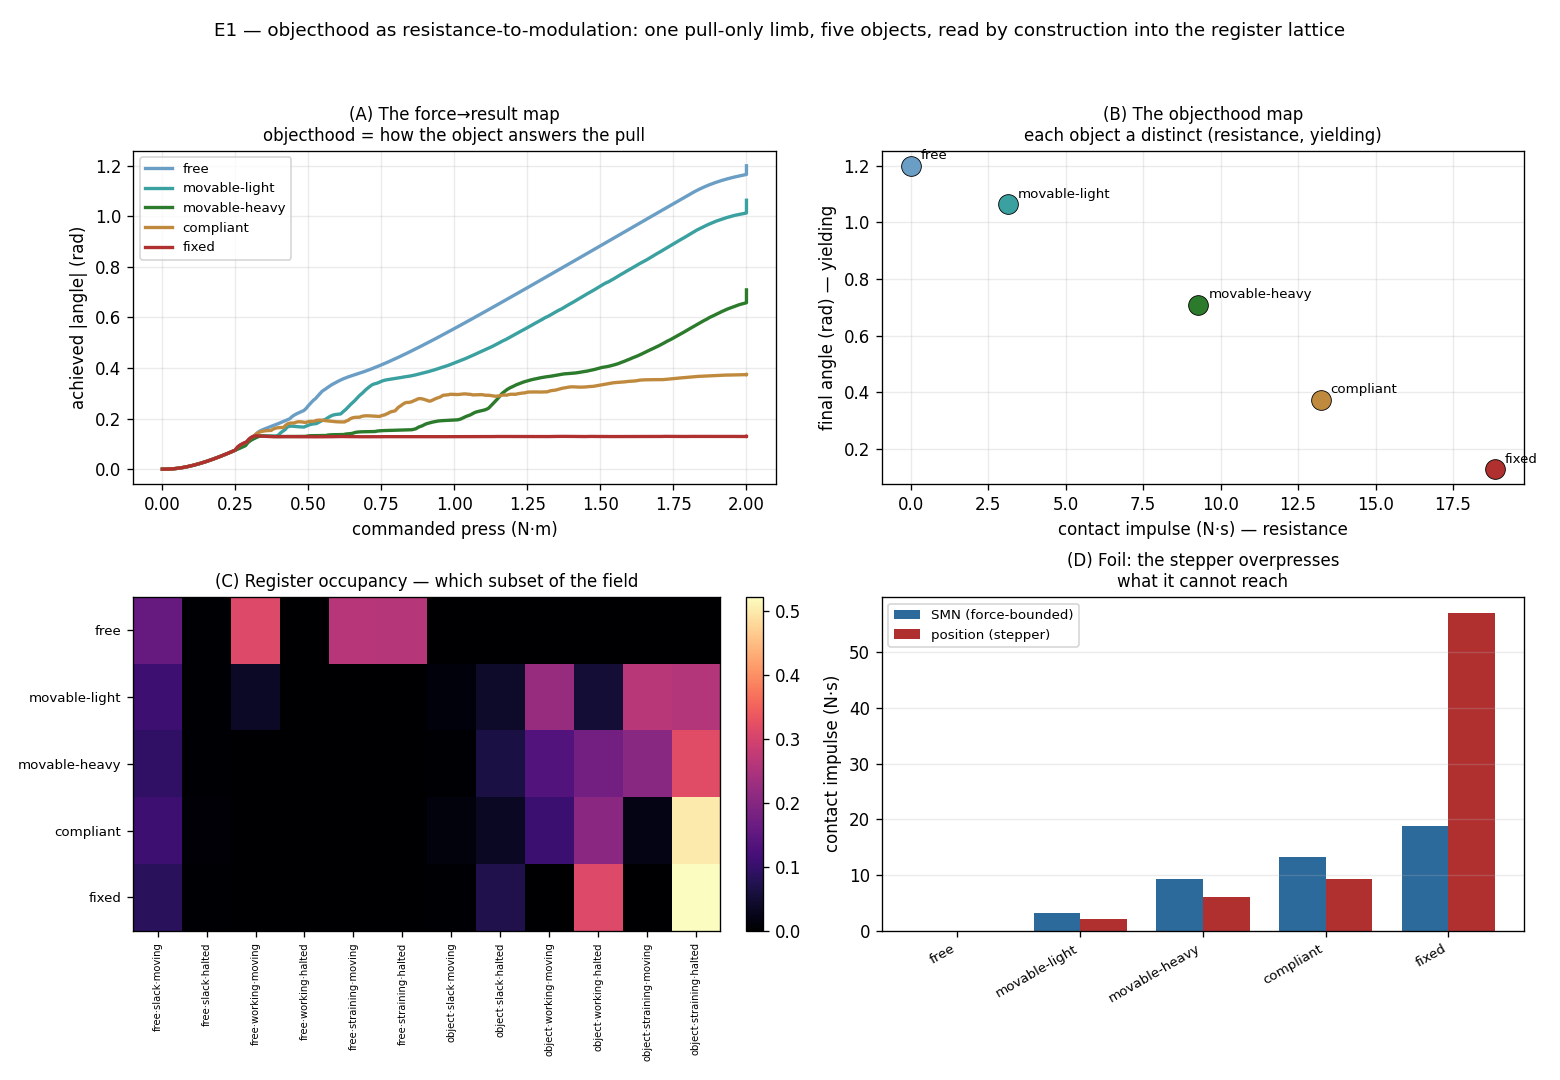
\includegraphics[width=\linewidth]{p4_manipulator_objecthood.png}
  \caption{\textbf{The single-zone difference register.} The force$\to$result map
  (A) and the (resistance, yielding) map (B) place five things on one arc;
  register occupancy is distinct per thing (C); the stepper foil overpresses the
  unreachable thing while the SMN pull stays force-bounded (D).}
  \label{fig:e1}
\end{figure}

\subsection{E2 --- self, field, and object}

A sagittal, gravity-loaded zone lifts against the field. By self-motion the agent
calibrates a \textbf{force-reafference} model --- the effort its own pull needs to
move the limb against gravity alone --- using the same reafference predictor that
gives the self/world register elsewhere in the bench, now in the force domain.
Thereafter the field is a predictable baseline; the residual (effort beyond it)
plus contact surface the object, and motion produced with no effort surfaces an
external cause. The three conditions are attributed correctly by construction
(Figure~\ref{fig:e2}): \emph{self+field} residual $\approx 0.001$, attributed
self+field with probability $1.00$; \emph{object} attributed $0.68$ (its
pre-contact phase honestly reading self+field) on a residual of $0.34$ plus
contact; \emph{external} attributed $1.00$. The self/world distinction is thereby
generalized into \textbf{self / field / object}, with the field --- gravity --- as
the always-present third term that, factored out, never masquerades as an object.

\begin{figure}[t]
  \centering
  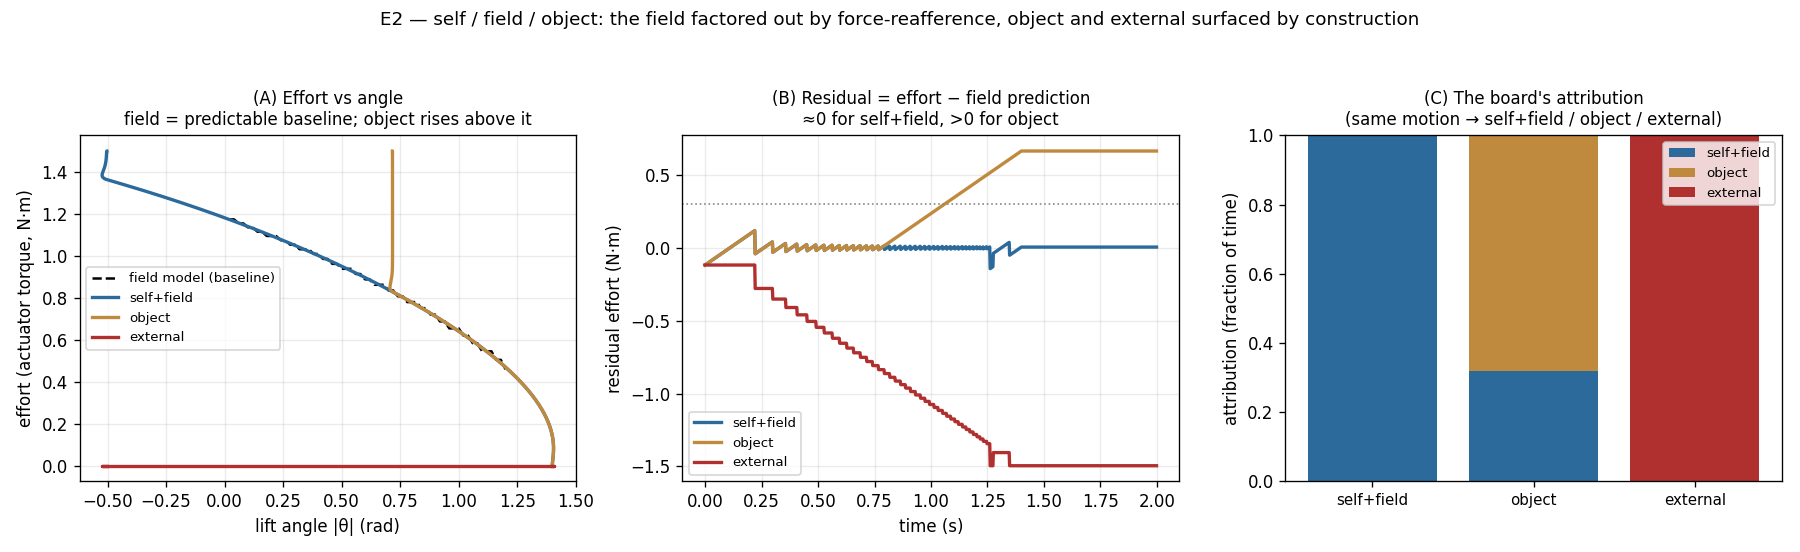
\includegraphics[width=\linewidth]{p5_self_field_object.png}
  \caption{\textbf{Self / field / object.} Effort versus angle against the
  calibrated field baseline (A); the residual beyond the field (B), $\approx 0$ for
  self+field and elevated for the object; the board's attribution (C).}
  \label{fig:e2}
\end{figure}

\subsection{E3 --- haltability generates aboutness}

A thing on the left; both limbs receive the same command. A halt-in-contact proves
to be a \emph{directed} state, not a stop (Figure~\ref{fig:e3}). It is
\textbf{persistent} --- the left zone sustains a directed halt for $1.51$\,s and
restores it after a perturbation knocks it off; \textbf{returnable} --- across
withdraw/re-press cycles the agent re-acquires the same thing five times; and
\textbf{side-specific} --- the right zone, given the identical command but nothing
to press, never holds ($0.00$\,s), so the left-halt/right-free asymmetry \emph{is}
directedness. A BAPG-only foil (basal rhythm without the haltable layer) only
flickers: its longest sustained halt is $0.26$\,s (seventeen brief touches),
because a rhythm is forced to release. Rhythm is not aboutness; haltability is.

\begin{figure}[t]
  \centering
  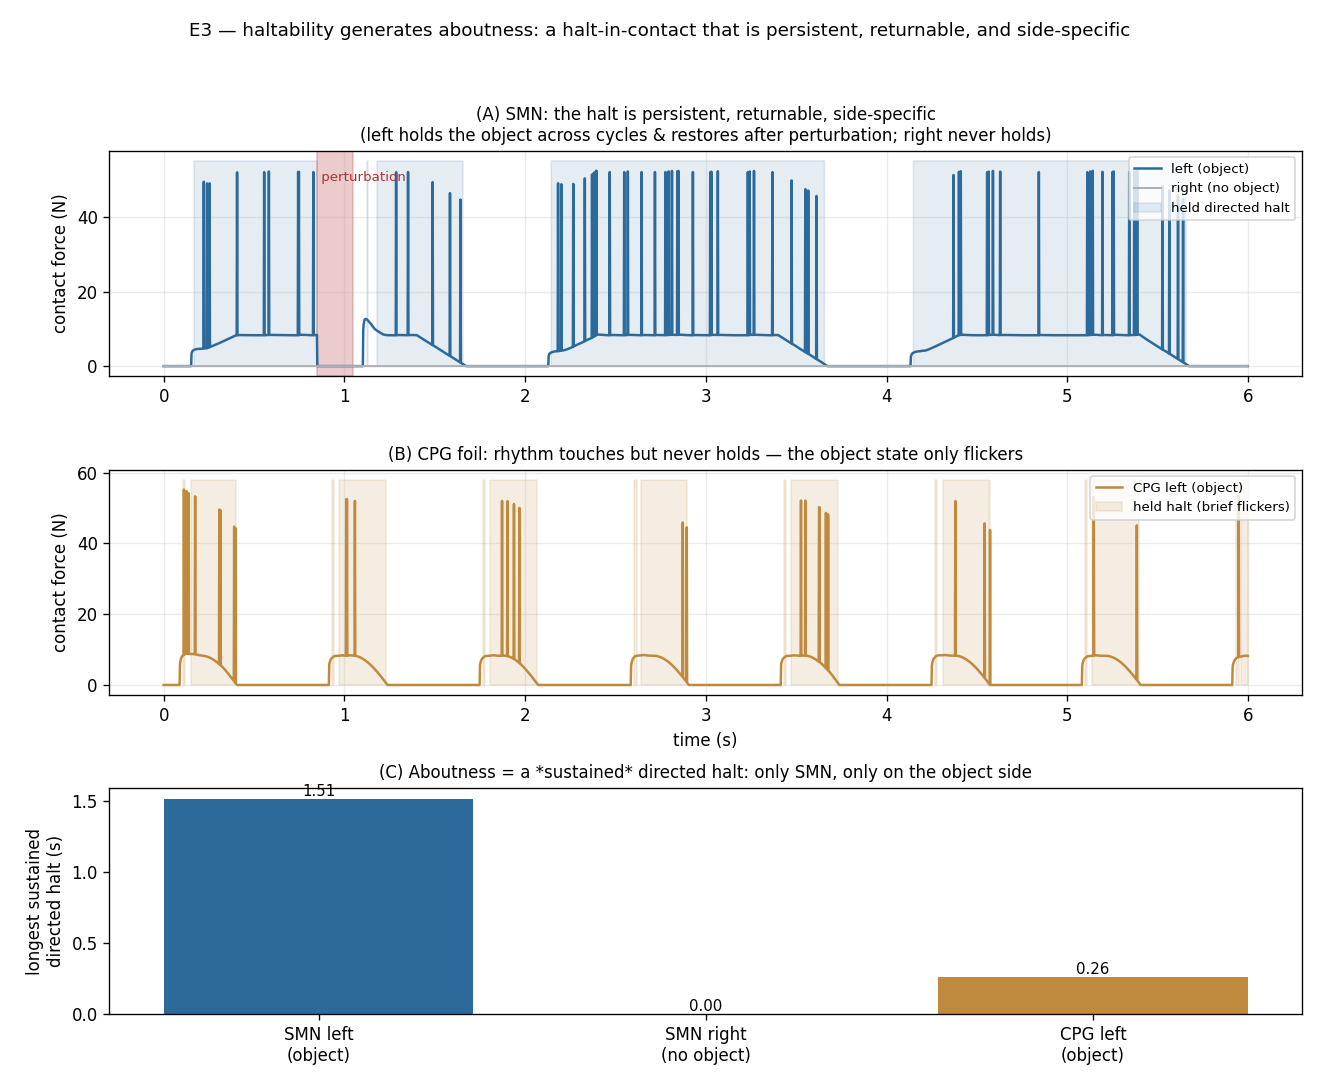
\includegraphics[width=\linewidth]{p6_haltability_aboutness.png}
  \caption{\textbf{Haltability generates aboutness.} The halt is persistent,
  returnable, and side-specific (A); a basal rhythm without the haltable layer can
  only flicker (B); a sustained directed halt is present only with haltability,
  only on the object side (C).}
  \label{fig:e3}
\end{figure}

\subsection{E4 --- objecthood as composition; the world model scales with the network}

A single zone gives a difference; an object is a \emph{composition} of differentiae,
which needs a \emph{network}. We make a row of $K$ pull-only antagonist
press-zones, each reading one facet's resistance differentia (hard vs.\ soft,
exactly as in E1), and let the board compose the bound zones into an object code.
We then measure the agent's world-model capacity --- the number of things it can
individuate --- as a function of how many zones the network binds.

The capacity scales as $2^{K}$ with the bound network (Figure~\ref{fig:e4}):
$2,4,8,16,32$ individuable objects for $K=1,\dots,5$, and \emph{every one} of the
$62$ composed objects is read correctly from real multi-zone presses
(per-object accuracy $1.00$; per-zone hard impulse $3.83$ vs.\ soft $2.08$). Zones
that are present but \emph{unbound} add nothing: a single difference, capacity
$2$, flat. The world model is built by the \emph{network}, not the sensor count
--- a clean scaling law, $\log_2(\text{capacity}) = (\text{bound zones})$. The
``object'' is exactly the composition of differentiae the coupled network can
hold; the BAPG floor fills the continuum between them, so the constructed world is
a smooth dynamical manifold, not a pixel grid.

\begin{figure}[t]
  \centering
  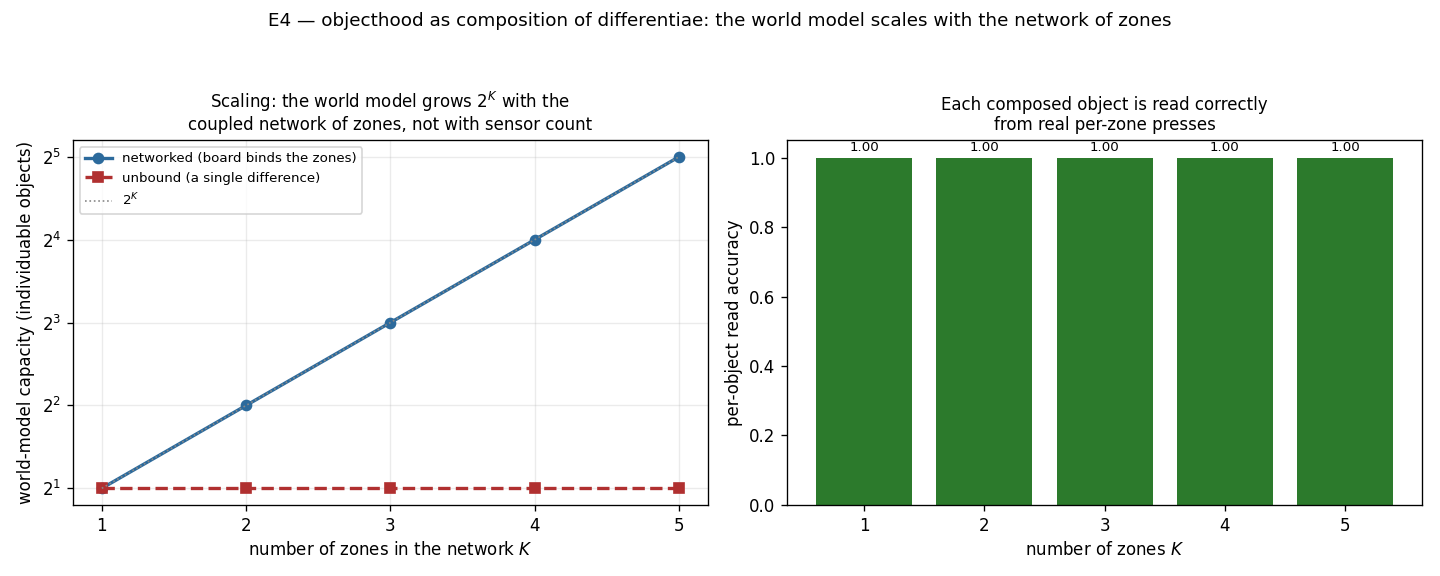
\includegraphics[width=0.92\linewidth]{p7_scaling_network.png}
  \caption{\textbf{The world model scales with the network of zones.} World-model
  capacity grows as $2^{K}$ with the coupled network (left), while unbound zones
  give only a single difference (capacity $2$, flat); each composed object is read
  correctly from real per-zone presses (right). Scaling the modulation is scaling
  the world.}
  \label{fig:e4}
\end{figure}

\subsection{E4b --- the onset of objecthood is a coupling-density transition}

Given reliable per-zone differentiae (E4), \emph{when} do they bind into an
object? Model the board as a random graph $G(K,p)$ --- each pair of zones coupled
with probability $p$ --- and let composition bind zones within a connected
component, so the richest single object the agent can hold is the largest bound
component, of capacity $2^{(\text{largest component})}$. Sweeping the coupling
density (Figure~\ref{fig:e4b}, $K=24$ zones), objecthood appears as a
\textbf{percolation-like transition}: below a critical density the differentiae
stay fragmented (the largest bound object a few zones, capacity $\sim 2^{4}$), and
past $p_c = 1/K$ a giant bound object emerges, the capacity jumping to $\sim
2^{18}$ by $p = 2/K$. The order parameter --- the largest bound object as a
fraction of $K$ --- is the classic giant-component curve. Objecthood, in this
architecture, is not all-or-nothing: it has a \emph{threshold} in the modulation
network's connectivity. (The per-zone differentiae here are the real bench reads
of E4; what is swept is the board's connectivity. This is the random-board
baseline; structured boards and the spectrum of the coupling matrix are the open
questions below.)

\begin{figure}[t]
  \centering
  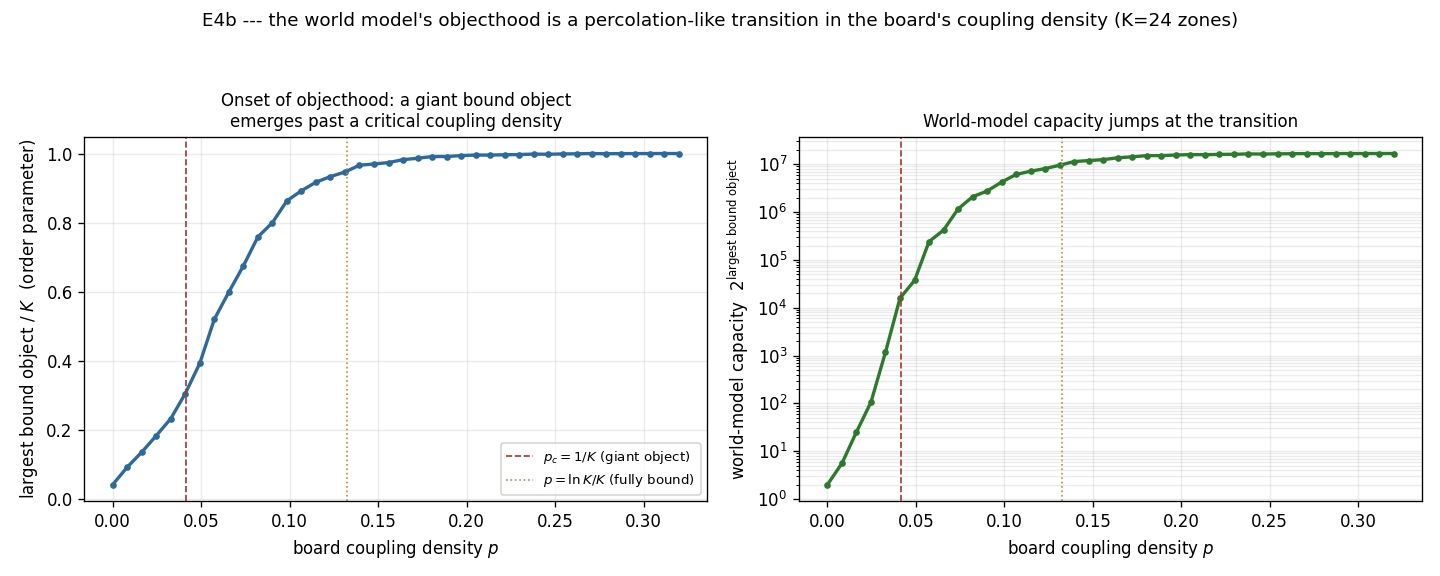
\includegraphics[width=0.92\linewidth]{p8_objecthood_transition.png}
  \caption{\textbf{Objecthood as a percolation transition.} The largest bound
  object (order parameter, left) and the world-model capacity (right) jump as the
  board's coupling density crosses $p_c = 1/K$: below it the differentiae are
  fragmented, above it a giant bound object emerges.}
  \label{fig:e4b}
\end{figure}

\section{Discussion}

The four results compose into one: \emph{the opponent-modulated body in a field
enacts, by construction, what learning or inference would otherwise supply --- and
the world it constructs scales with the network that binds its differentiae.} A
single zone registers a difference (E1) that already carries a self/field/object
factoring (E2) and a haltable aboutness (E3); an object is the composition of such
differences across coupled zones, and the agent's world-model capacity grows
$2^{K}$ with the bound network (E4). Nothing is learned, and nothing inverts an
internal model; the structuring prior is the physics the body is coupled to, and
the structuring \emph{degrees of freedom} are the couplings of the board.

This places us precisely among neighbours. With \citet{Gardenfors2014,Gardenfors2020}
we share the geometry and the two-vector, force-based account of events; we differ
in enacting the force$\to$result mapping rather than learning it, and we would
offer one refinement of his cognitivism --- the \emph{forces} are physically real,
while the \emph{objecthood} read off them is constructed. This is
\citeauthor{Smith1996}'s middle course between realism and constructionism in
concrete form: the flux is real; the object is wrestled from it by the agent's
modulation, and is exactly as rich as the network can compose. With active
inference \citep{ParrPezzuloFriston2022} we share a single principle doing
first-principle work; we differ in locating the prior in the world--body coupling
--- gravity as a free prior, read through the work the agent does against it ---
rather than in a represented model. Whether ``minimize prediction error'' and
``compensate against the field'' are two descriptions of one event is, to us, an
open and inviting question.

The scaling result reframes the agent as a \textbf{complex network} and opens
genuinely physical questions that our cognitive vocabulary cannot answer. E4b
already shows the baseline: for a \emph{random} board, objecthood appears at the
giant-component threshold $p_c = 1/K$. What remains open is squarely physics: how
do \emph{structured} boards --- modular, hierarchical, scale-free --- shift that
onset; \emph{what does the spectrum} of the coupling matrix say about which
networks compose objects (a random-matrix question); and what are the dynamics of
binding? The bench supplies the coupling matrices and trajectories to ask them.
The geometry of the
constructed world is itself body-indexed: its dimensionality is set by the network
(the number of bound zones), its coordinates by the agent's own configuration ---
so morphology fixes the geometry of the world an agent can have.

The account is bounded. The $2^{K}$ law is, once each facet is one clean bit,
true by construction; the non-trivial content is the \emph{dissociation} (capacity
tracks the bound network, not the raw sensor count) and a real multi-zone body
reading $62$ objects without error. The held halt is supplied by the object plus
continued press; a \emph{free-space} co-contraction equilibrium with tunable
stiffness needs muscle/tendon actuators (ideal torque motors make co-contraction
inert). Unifying the horizontal and gravity-loaded variants on one body, chaining
zones into a crawler that builds a habitat-scale model, and the coupling-density
transition above, are the next steps. \emph{Naming} --- a shared symbol for the
composed object --- is conventional and social and lies beyond a single agent.

\section{Reproducibility}

The bench, the units, and an interactive interface are open
(\texttt{github.com/gnowgi/smn-lab}, GPL-3.0). Each result is produced by a single
seeded script (the E1--E4 experiments) and the figures regenerate from them; the
register lattice and the coupling matrix are computable from the body's structure
alone. A versioned snapshot with a Zenodo DOI will accompany the published
version.

\section{Conclusion}

In an embodied Sensation Modulating Network, objecthood is a composition of
differentiae: a single zone registers a difference --- resistance, with its
self/field/object factoring and its haltable aboutness --- and an object is what a
coupled \emph{network} of zones composes. The world an agent can construct scales
with that network, $2^{K}$ in the zones it binds, and emerges --- as the coupling
density rises --- at a percolation threshold. Scaling the modulation is scaling
the world; the architecture, not a corpus or an inferred model, is doing the work.

\bibliographystyle{plainnat}
\bibliography{references}

\end{document}
